\documentclass[a4paper, 11pt, titlepage]{scrartcl} %scrartcl f�r kurze Artikel

% \renewcommand*\sectfont{\normalcolor\rmfamily\bfseries}
% \renewcommand*\descfont{\rmfamily\bfseries}
% \setkomafont{dictum}{\normalfont\normalcolor\rmfamily\small}

\makeatletter% siehe De-TeX-FAQ
\renewcommand*{\toc@heading}{%
  \addsec{\contentsname}% bei scrartcl \addsec statt \addchap
  \@mkboth{\contentsname}{\contentsname}%
}
\makeatother% siehe \makeatletter

\usepackage[ngerman]{babel}
\usepackage[ansinew]{inputenc}
\usepackage[T1]{fontenc}
\usepackage{lmodern}
% \usepackage{times}
% \usepackage{mathptmx}
\usepackage{color}
% \usepackage{courier} % Monospace/Truetype umstellen
\usepackage{enumitem} % \begin{enumerate}[label={\alph*)}] \item \end{enumerate} f�r a) b) c)...
\usepackage{rotating}
\usepackage{grffile}
\usepackage{amsmath}
\usepackage{amssymb}
\usepackage{subfig}
\usepackage{setspace}
\setcapindent{0em} 
\interfootnotelinepenalty=10000
\raggedbottom
\usepackage{algorithm}
\usepackage{algorithmic}
	\renewcommand{\algorithmiccomment}[1]{// #1}
\usepackage{ulem}
	\normalem %stellt emph{} wieder auf kursiv, sonst unterstrichen
\usepackage{graphicx}
\graphicspath{{img/}}
\usepackage[hmargin={3cm,2cm}, vmargin={2cm, 3cm}]{geometry}
\usepackage{nicefrac} 	
\usepackage{titlesec}
\titlespacing{\section}{0pt}{*6.5}{*1.5}
\titlespacing{\subsection}{0pt}{*2}{*1}
\titlespacing{\subsubsection}{0pt}{*1}{*0.5}
\bibliography{literature}
\usepackage[style=authoryear]{biblatex} 
\addbibresource{literature.bib}

\DefineBibliographyStrings{ngerman}{
    references = {Literaturverzeichnis}
}

\defbibenvironment{bibliography}
{\list{}
{\setlength{\leftmargin}{\bibhang}%
\setlength{\itemindent}{-\leftmargin}%
\setlength{\itemsep}{12px}%
\setlength{\parsep}{\bibparsep}}}
{\endlist}
{\item}
\ExecuteBibliographyOptions{dashed=false}

%use for code formatting
\newcommand{\code}[1]{\texttt{#1}}

\tolerance=500

\renewcommand{\topfraction}{0.7}	% max fraction of floats at top

\usepackage{url}
\urlstyle{leo}

% Punkt + Komma Abst�nde bei Tausendern/Dezimalzahlen ans dt. anpassen
% \mathcode`,="013B
% \mathcode`.="613A

%\usepackage{hyperref}
\usepackage{csquotes}
\usepackage{parcolumns}

% \bibliography{literature}
% \usepackage[style=numeric, autocite=inline, labelnumber=true]{biblatex} 
% \addbibresource{literature.bib}
% 
% \DefineBibliographyStrings{ngerman}{
%     references = {Literaturverzeichnis}
% }
% 
% \defbibenvironment{bibliography}
% {\list{}
% {\setlength{\leftmargin}{\bibhang}%
% \setlength{\itemindent}{-\leftmargin}%
% \setlength{\itemsep}{12px}%
% \setlength{\parsep}{\bibparsep}}}
% {\endlist}
% {\item}

\usepackage{parskip}

% \parindent 0pt %Absatzeinr�ckung
% \parskip 12pt %Absatzabstand

\begin{document}

\label{Titelseite}

\begin{titlepage}
\begin{center}

\ 

\vspace{2\baselineskip}

Martin-Luther-Universit�t\\
Halle-Wittenberg

\vspace{\baselineskip}

-- Juristische und Wirtschaftswissenschaftliche Fakult�t --

\vspace{\baselineskip}


\includegraphics[width=6cm]{mlu}

\vspace{\baselineskip}

\textbf{Projektarbeit}

\vspace{\baselineskip}

\renewcommand{\baselinestretch}{1.4}\normalsize
\textbf{\Large{Krankheitsausbreitung in Bienenpopulationen}}

\renewcommand{\baselinestretch}{1.00}\normalsize
\vspace{\baselineskip}

\parbox{0cm}{
\begin{tabbing}
XXXXXXXXXXXXXXXX\= \kill \\ 
Lehrveranstaltung:\> Simulation - Techniken und Software\\
\\
Dozenten:
\> Prof. Dr. Ta\"{\i}eb Mellouli\\
\> Michael R�mer \\
\\
Abgabetag: \>16. glaube ich oder 19.
\end{tabbing}}

\vspace{3\baselineskip}

\parbox{0cm}{
\begin{tabbing}
XXXXXXXXXXXXXXXXXXXXXXX\= \kill \\
Sebastian B�r\>2. Semester Master\\
Bugstehude\> Matr.-Nr. 209213003\\
01234 XXXX\>Wirtschaftsinformatik
\end{tabbing}
}

\parbox{0cm}{
\begin{tabbing}
XXXXXXXXXXXXXXXXXXXXXXX\= \kill \\
Daniel Haake\>2. Semester Master\\
Bugstehude\> Matr.-Nr. 012345678\\
01234 XXXX\>Wirtschaftsinformatik
\end{tabbing}
}

\parbox{0cm}{
\begin{tabbing}
XXXXXXXXXXXXXXXXXXXXXXX\= \kill \\
Frank Rosner\>2. Semester Master\\
Goethestra�e 3\> Matr.-Nr. 209211038\\
06114 Halle\>Wirtschaftsinformatik
\end{tabbing}
}

\end{center}
\end{titlepage}


\renewcommand{\baselinestretch}{1.4}\normalsize

\pagenumbering{Roman} \setcounter{page}{2}

% \setcounter{page}{0}\clearpage\newpage
\renewcommand{\baselinestretch}{1.25}\normalsize

\addcontentsline{toc}{section}{Inhaltsverzeichnis}
\tableofcontents

\renewcommand{\baselinestretch}{1.4}\normalsize

\newpage

% \addcontentsline{toc}{section}{Abbildungsverzeichnis}
% \listoffigures
% 
% \newpage
% 
% \section*{Abk�rzungsverzeichnis}
% \addcontentsline{toc}{section}{Abk�rzungsverzeichnis}
% 
% \begin{tabular}{ll}
% \LSH & Locality Sensitive Hashing\\
% \WDM & Wort-Dokument-Matrix
% \end{tabular}
% 
% \newpage
% 
% \listoftables
% \addcontentsline{toc}{section}{Tabellenverzeichnis}
% 
% \newpage

\renewcommand{\baselinestretch}{1.5}\normalsize
\pagenumbering{arabic} \setcounter{page}{1}

\section{Einleitung}



\newpage

\section{Simulationsmodell}

Um die Best�ubung seiner der Ackerfl�chen sicherzustellen, erteilt ein Bauer einem Imker einen Best�ubungsauftrag. Dem Imker steht die Ackerfl�che zur Verf�gung um seine Bienenst�cke zu platzieren, damit die Best�ubung optimal stattfinden kann. In der Simulation wirken der Imker, die Bienenst�cke mit Bienenpopulationen, die Krankheit und die Blumen zusammen.

Innerhalb eines Stocks gibt es eine K�nigin, Arbeiter und Drohnen. Jeder Bienenstock hat eine K�nigin, die solange neue Eier legt, bis die Kapazit�t des eigenen Stocks erreicht ist. Ein Arbeiter fliegt zu Blumen, um eine Menge von Nektar zu sammeln und diesen zur�ck in den Bienenstock zu bringen. Nach einem Sammelvorgang ruht sich die Biene aus. Arbeiter k�nnen unbeabsichtigt zu einem fremden Stock fliegen. Dort geben sie den Nektar ab und werden danach ausgesto�en. Eine Biene stirbt nach einer bestimmten Zeit eines nat�rlichen Todes oder verendet durch die Krankheit. Ein Bienenstock kollabiert, falls eine bestimmte Anzahl lebender Bienen unterschritten wurde.

Bienen k�nnen sich mit der Krankheit infizieren. Falls sich eine Biene angesteckt hat, kann sie die Krankheit auf weitere Bienen �bertragen. Eine �bertragung kann entweder innerhalb eines Stocks oder beim Zusammentreffen zweier Bienen an einer Bl�te geschehen. Zwischen der Infizierung einer Biene mit der Krankheit und dem Ausbruch liegt eine bestimmte Zeit.

Die Blumen sind gleichm��ig �ber die Fl�che verteilt. Jede Blume verf�gt �ber eine Menge von Nektar. Nachdem der Nektar entnommen wurde, dauert es eine bestimmte Zeit bis sich der Vorrat wieder auff�llt.

Das Ziel der Simulation ist herauszufinden, ob die Platzierung der Bienenst�cke Einfluss auf die Zeitdauer bis zum Kollaps aller Bienenpopulationen eines Imkers hat. Dazu soll die Zeitdauer bis zum Kollaps unter verschiedenen Platzierungsszenarien gemessen werden.

Zur Vereinfachung des Modells wurden bestimmte Annahmen getroffen. So entf�llt die explizite Unterscheidung zwischen Drohnen und Arbeitern. Es wird davon ausgegangen, dass ein bestimmter Prozentsatz der Bienen sich immer innerhalb des Stocks aufh�lt. Um einen Krankheitsausbruch abzubilden, ist am Anfang eines Simulationslaufs ein bestimmter Teil der Bienen erkrankt.

Um eine Verzerrung der Outputgr��en zu unterbinden, werden alle Bienenst�cke zu Beginn einer Simulation mit einer zuf�lligen Bienenpopulation ausgestattet. D.h. in jedem Stock ist bereits eine Anzahl von Bienen vorhanden, die sich in unterschiedlichen Lebensabschnitten befinden.

Die Simulation ist dynamisch und ereignisdiskret. Das System wird �ber einen bestimmten Zeitraum betrachtet und der Zustand des Systems �ndert sich durch das Eintreten bestimmter Ereignisse. Solche Ereignisse w�ren beispielsweise: das Schl�pfen und Sterben einer Biene, das Losfliegen zu einer Bl�te oder die Ansteckung einer Biene mit der Krankheit. Als Inputdaten werden teils Daten aus wissenschaftlichen Ver�ffentlichungen, teils durch Sensitivit�tsanalysen ermittelte Daten benutzt. Die Simulation endet, wenn alle Bienenpopulationen kollabiert sind.


\section{Implementierung}

Zur Umsetzung der Simulation verwenden und erweitern wir das Java Framework \emph{Tortuga}\footnote{\texttt{http://code.google.com/p/tortugades/}}, welches die grundlegenden Funktionalit�ten einer ereignisdiskreten Simulation anbietet. Mit Hilfe aspektorientierter Programmierung wird gew�hrleistet, dass innerhalb des Programmcodes der selbstdefinierten Entit�tsklassen jederzeit Zugriff auf die Simulation m�glich ist um beispielsweise ein neues Ereignis zu registrieren, damit es in die Ereignisliste eingef�gt wird.\footnote{N�heres zum Thema aspektorientierter Programmierung kann der geneigte Leser zum Beispiel \textcite{kiczales1997aspect} entnehmen. \textcite{laddad2003aspectj} beleuchtet die AspectJ-Erweiterung f�r aspektorientiertes Programmieren in Java genauer.}

Basisklassen f�r eine Simulation und Entit�ten sind in Tortuga vorhanden, wobei die abstrakte Klasse \code{org.mitre.sim.DefaultEntity} vom Frame\-work\-nutzer erweitert werden muss. Abbildung~\ref{img:entities} zeigt ein UML-Klassendiagramm der Entit�tshierarchie unserer Simulation. Um Bewegungen im zweidimensionalen Raum zu erm�glichen, wird zun�chst die \code{DefaultEntity} um Positionsdaten erweitert. Die entstehende abstrakte Klasse \code{PositionedEntity} bietet bereits eine erste ereignisausl�sende Methode an: \code{moveTo(Position, double)}. Beim Aufruf dieser Methode wird das Ereignis \code{arriveAt(Position)} f�r das Ende der angegebenen Bewegungszeit bei der Simulation registriert, also in die Ereigniswarteschlange eingef�gt. Es �ndert dann beim Eintreten die Position der Entit�t.

Ereignisse werden in Tortuga als gew�hnliche Methoden deklariert und bei der Simulation mit Methodennamen und Parametern registriert. Das Framework ruft die Methoden zur entsprechenden Simulationszeit �ber die \emph{Java Reflection API}\footnote{Die Java Reflection API kann unter anderem verwendet werden, um Klassen oder Methoden aufzurufen, die zur Compiletime noch unbekannt sind. Sie m�ssen somit erst zur Laufzeit vorhanden sein. N�here Informationen finden sich auf \texttt{http://docs.oracle.com/javase/tutorial/reflect/}.} auf.

F�r unsere Simulation werden drei konkrete \code{PositionedEntity} Klassen ben�tigt: Bienenst�cke, Bienen und Blumen. Abbildung~\ref{img:entities} zeigt die entsprechenden Klassen.

\begin{figure}[t]
	\begin{center}
    	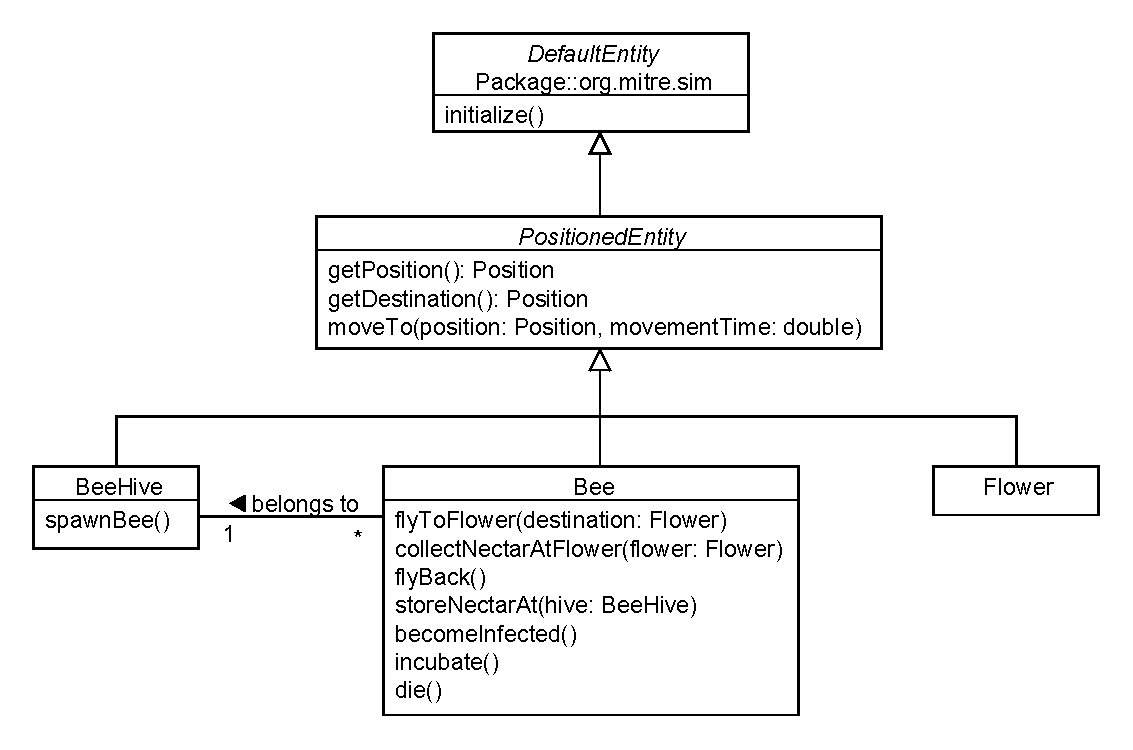
\includegraphics[width=1\linewidth]{entities}
  \caption{UML-Klassendiagramm der Simulationsentit�ten. Auf die Darstellung privater und nicht simulationsbezogener Methoden und Attribute wird aus �bersichtlichkeitsgr�nden verzichtet. Die Klasse \code{DefaultEntity} wird vom Simulationsframework Tortuga bereitgestellt.}
  \label{img:entities} 
	\end{center}
\end{figure}

\begin{description}
\item[Bienenst�cke] beherbergen die Bienen, die zur aktuellen Simulationszeit lebendig sind. Das Ereignis \code{spawnBee()} wird periodisch ausgef�hrt. Es erstellt, sofern der Stock noch Kapazit�ten hat, eine neue Biene und simuliert das Eierlegen der K�nigin.
\item[Bienen] erledigen das Sammeln des Nektars. Die Simulation l�st \code{flyToFlower(Flower)} aus, wenn die Biene sich eine neue Blume zum Nektar sammeln suchen soll. Anschlie�end wird die \code{moveTo}-Methode aufgerufen und \code{collectNectarAtFlower(Flower)} f�r die Ankunft an der Blume in die Ereignisliste eingef�gt.

Nach dem Sammeln des Nektars an der Bl�te entscheidet sich die Biene, ob sie noch Kapazit�t f�r weiteren Nektar hat oder zur�ck zum Stock fliegt um den Nektar abzuladen. Falls sie weitere Blumen anfliegen m�chte, l�st sie wieder \code{flyToFlower(Flower)} aus. Anderenfalls wird \code{flyBack()} ausgel�st, welches die Biene bewegt und f�r die Ankunft \code{storeNectarAt(Hive)} registriert. Sollte sich die Biene verfliegen, ist der als Parameter �bergebene Bienenstock ein anderer als der Heimatstock der Biene.

Bei Kontakt mit anderen Bienen im Stock oder an einer Bl�te kann eine Ansteckung stattfinden. Mit einer bestimmten Wahrscheinlichkeit wird, falls eine der beiden Bienen an der selben Position krank ist, das Ereignis \code{becomeInfected()} aufgerufen. Dort wird die restliche Lebenszeit der angesteckten Biene verringert und die Inkubationszeit beginnt. F�r den Ablauf der Inkubationszeit reiht sich das Ereignis \code{incubate()} in die Ereignisliste ein, sodass andere Bienen die Infektion bemerken k�nnen.

Nach Ablauf der normalen Lebenszeit oder am Ende des Krankheitsverlaufes sterben Bienen, indem das Ereignis \code{die()} ausgef�hrt wird.
\item[Blumen] dienen den Bienen als Nektarlieferanten. Sie haben keine Ereignisse, da ihr Nektar �ber die Simulation zentral erneuert wird. Blumen bleiben f�r den gesamten Simulationszeitraum bestehen.
\end{description}

Damit Bienen die Blumen in ihrer Umwelt sehen k�nnen sind alle aktiven Entit�ten der Simulation in einer \code{Environment} registriert. Die \code{Environment} zeigt den Bienen verf�gbare Blumen und k�mmert sich um das Erneuern des Nektars aller Bl�ten.




\section{Experimente}
\label{sec:experiments}

Das Ziel der Experimente war die �berpr�fung, ob die Art und Weise der Platzierung der Bienenst�cke einen Einfluss auf die Ausbreitungsgeschwindigkeit des ABPV. Der Einfluss wurde �ber die Zeitdauer gemessen, bis alle Bienen ausgestorben waren. So wird eine Platzierungsstrategie einer anderen vorgezogen, wenn die Zeit bis zum Ableben aller Bienen der einen gr��er ist als bei der anderen.

\subsection{Eingabegr��en}

Viele Eingabegr��en der Simulation stammen aus \textcite{tautz2007phaenomen}, \textcite{genersch2010honey} und \textcite{tautz2013bee}. Gr��en, die keiner verl�sslichen Quelle entnommen werden konnten, wurden durch eine Sensitivit�tsanalyse gew�hlt. Eine exakte Auflistung der verwendeten Eingabegr��en findet sich in Tabelle~\ref{tab:inputs}.

%Tautz und Heilmann (2007): Informationen zu Biene, Stock und Bl�te
%- Rollen der Bienen im Stock (K�nigin, Sammler, Arbeiter)
%- Beziehung der Biene zur Bl�te (Bl�te als zentrales Element im Leben einer Biene)
%
%Genersch (2010): Inhalte zu Krankheitserregern
%- verschiedenste Arten von Erregern werden abgehandelt (Parasiten, Viren, Bakterien)
%- Wirkungsweise und Auswirkung auf Bienen(populationen))
%
%Tautz (2013) hobos.de: Allgemeine Informationen
%- Stock Funktionalit�ten
%- Gr��e und Verhaltensweisen der Bienen im und au�erhalb des Stocks
%- Flugweiten der Bienen
%- Wie orientieren und verhalten sich Bienen im Flug
%Sehr viele unterschiedliche Inhalte. Querschnitt �ber die Biene als Organismus und deren Sozialverhalten (Stock)

\vspace*{1em}
\begin{table}[h]
\begin{minipage}[t]{0.48\linewidth}
	\begin{center}
	\begin{tabular}{lr}
	\textbf{Bienen} & \\ \hline
	Fluggeschwindigkeit & 5\,\nicefrac{km}{h} \\
	Nektartragekapazit�t & 40\,mg\\
	Dauer des Nektarsammelns & 0{,}5\,m \\
	Dauer des Stockaufenthalts & 5\,h \\
	maximaler Verfliegeradius & 200\,m \\
	Lebensdauer ($\mu$) & 45\,d \\
	Lebensdauer ($\sigma$) & 5\,d \\
	Lebensdauer nach Erkrankung & 4\,d \\
	Infektionswahrscheinlichkeit & 0{,}05\,\% \\
	Inkubationszeit & 2\,d
	\end{tabular}
	\end{center}
\end{minipage}
\hspace*{0.02\linewidth}
\begin{minipage}[t]{0.48\linewidth}
	\begin{center}
\begin{tabular}{lr}
\textbf{Bienenstock} & \\ \hline
Anzahl Bienen pro Stock & 1000 \\
Eierlegerate & 43{,}2\,s \\
Anteil Arbeiterbienen & 55\,\% \\
initiale Erkrankungsrate & 0{,}1\,\% \\
Kollabierungsschwellwert & 75\,\% \\
\\
\textbf{Blumen} &  \\ \hline
Anzahl Blumen pro Biene & 8 \\
Nektarmenge pro Blume & 16\,mg \\
Dauer der Nektarregenerierung & 1\,d
\end{tabular}
	\end{center}
\end{minipage}
\begin{center}
\caption{Eingabegr��en der Simulation, geordnet nach zugeh�rigem Entit�tstyp.}
\label{tab:inputs}
\end{center}
\end{table}

Ein Bienenstock beherbergt normalerweise ungef�hr 50{.}000 Bienen. Aufgrund implementierungstechnischer Beschr�nkungen durch das verwendete Simulationsframework musste diese Gr��e auf 1000 Bienen pro Stock reduziert werden. Eine Bienenk�nigin legt ca. 2000 Eier pro Tag. Das entspricht einer Legerate von einem Ei alle 43 Sekunden. Der Anteil der Sammlerbienen betr�gt 55\,\%. 

Eine Biene lebt im Durchschnitt 45 Tage. Um nat�rliche Lebensdauerschwankungen zu modellieren, nehmen wir eine Normalverteilung $\mathcal N(\mu, \sigma)$ der Lebensdauer mit $\mu = 45$ und $\sigma = 5$ an. Die Zeit, die eine Sammlerin zum Nektarsammeln ben�tigt, wird mit einer halbe Minute angenommen. Nachdem eine Biene zu ihrem Stock zur�ckkehrte, gibt sie den Nektar ab und ruht sich danach aus. Es wird eine Aufenthaltsdauer von f�nf Stunden angenommen, bis die Biene erneut losfliegt. 

Bienen bewegen sich im Flug mit 5\,\nicefrac{km}{h} fort und k�nnen 40\,mg Nektar transportieren. Die Wahrscheinlichkeit, dass beim R�ckflug der Heimatstock nicht gefunden wird (die Biene sich verfliegt) h�ngt von der r�umlichen N�he des fremden Stockes ab. Je n�her ein fremder Stock dem Heimatstock ist, desto gr��er ist die Verfliegwahrscheinlichkeit. St�cke, die weiter als 200\,m vom Heimatstock entfernt sind, k�nnen nicht ausgew�hlt werden.

Zu Beginn der Simulation sind 0{,}1\,\% der Bienen erkrankt. Das entspricht ungef�hr einer Biene pro Stock. Die Ansteckungswahrscheinlichkeit\footnote{Die Ansteckungswahrscheinlichkeit ist in der Natur erheblich h�her. Jedoch kann eine Ansteckung nur stattfinden, wenn sich zwei Bienen ber�hren. In unserem Modell wird keine Ber�hrung simuliert und eine Biene kann theoretisch jede andere an der gleichen Position (Bl�te oder Stock) anstecken. Somit ist die von uns modellierte Ansteckungswahrscheinlichkeit genauer gesagt die Wahrscheinlichkeit f�r das zuf�llige Ber�hren zweier Bienen gefolgt von einer Ansteckung.} wurde so gew�hlt, dass die Populationen eine l�ngere Zeit �berleben, aber trotzdem nach gewisser Zeit alle St�cke kollabieren. Bei Wahrscheinlichkeiten kleiner als 0{,}05\,\% �berleben einige St�cke. Ist die Wahrscheinlichkeit gr��er, sterben die Bienen alle nach ungef�hr vier Tagen. Sobald 75\,\% der Bienen eines Stocks infiziert sind, kollabiert der ganze Stock. Die Inkubationszeit betr�gt zwei Tage. Insgesamt �berlebt eine infizierte Biene maximal vier Tage.

Die Anzahl der Blumen pro Biene wurde so angenommen, dass die Blumen zu jeder Zeit �ber Nektar verf�gen und es zu keinen Engp�ssen kommt. Nach Beginn der Simulation pegelt sich der verf�gbare Nektar bei ungef�hr 50\,\% der Gesamtkapazit�t aller Bl�ten ein. Eine Blume regeneriert 1\,mg Nektar pro Tag (Annahme).

\subsection{Stellgr��e und Simulationsszenarien}

Das Platzieren der Bienenst�cke geschieht folgenderma�en: Die Bienenst�cke werden in Gruppen unterteilt, die mit gr��tm�glicher Entfernung zueinander platziert werden. Innerhalb der Gruppen werden die enthaltenen St�cken direkt nebeneinander angeordnet. Bei gegebener Anzahl der St�cke werden verschiedene Anzahlen von Gruppen und Gruppengr��en simuliert. In der nachfolgenden Abbildung~\ref{img:summary} wird die Anzahl der Gruppen durch \textbf{n} und die Bienenst�cke pro Gruppe durch \textbf{s} symbolisiert.

\begin{figure}[t]
	\begin{center}
    	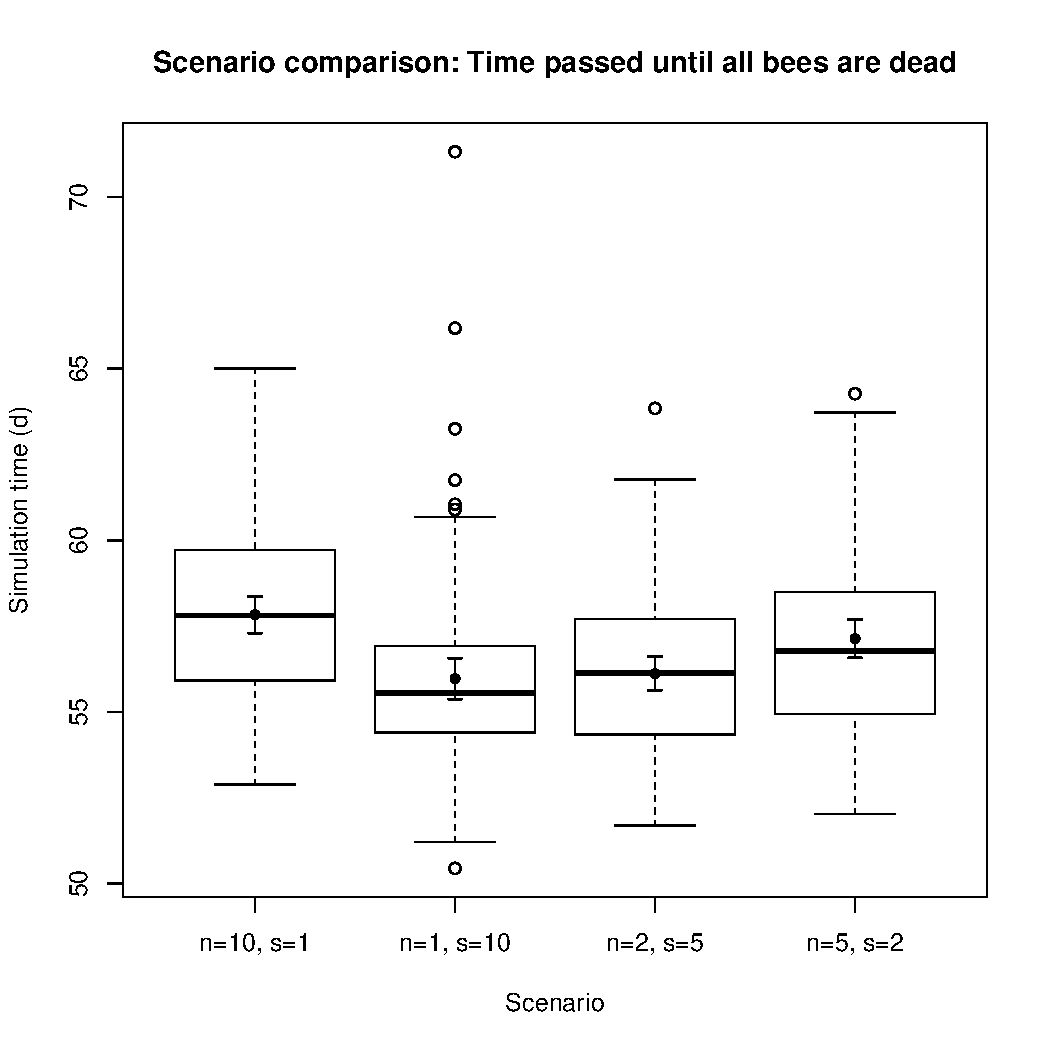
\includegraphics[width=1\linewidth]{summary}
  \caption{Zeitdauer bis zum Absterben aller Bienen, wobei $n$ die Anzahl der Gruppen und $s$ die Bienenst�cke pro Gruppe bezeichnet.}
  \label{img:summary} 
	\end{center}
\end{figure}

Bei einem Simulationslauf mit 100 Repetitionen pro Konfiguration l�sst sich erkennen, dass die Platzierung mit einem Stock pro Gruppe eine h�here Lebensdauer besitzt als alle anderen. Das deutet darauf hin, dass die Platzierung der St�cke mit gr��tm�glicher Entfernung zu einander geschehen sollte. Auff�llig ist, dass bei der Wahl von $n=1$ und $s=10$ die Anzahl der Ausrei�er �u�erst gro� ist. \textbf{mehr!}


\section{Schlussbetrachtung}

Das Finden von korrelierten W�rtern in gro�en Dokumentsammlungen ist eine wichtige Zutat f�r das Analysieren von Texten. Kommen zwei W�rter h�ufig gemeinsam in einzelnen Dokumenten einer Sammlung vor, so weisen sie eine hohe Korrelation auf. Solche korrelierten W�rter k�nnen verwendet werden, um automatisiert Thesauri zu erzeugen (\cite{baeza1992introduction,lin1998automatic,lassi2002automatic}). Das Finden von Synonymen ist ebenfalls eine wichtige Anwendung des Textminings (\cite{turney2001mining}).

Zur Bestimmung hoher Wortkorrelationen einer Dokumentsammlung kann eine Korrelationsmatrix mit den paarweisen Korrelationen aller W�rter berechnet werden, aus der anschlie�end die hohen Korrelationen extrahiert werden. Beinhalten Dokumentsammlungen viele Dokumente und W�rter, ist dies jedoch auf Grund des quadratischen Rechenaufwandes kaum noch m�glich. Um dennoch in der Lage zu sein, hohe und damit interessante Wortkorrelationen zu bestimmen, l�sst sich eine von \textcite{indyk1998approximate} entwickelte Technik zum Finden �hnlicher Objekte im hochdimensionalen Raum, das sogenannte Locality-Sensitive-Hashing (LSH), anwenden. \textcite{charikar2002similarity} hat ein spezielles LSH-Schema entwickelt, welches das effiziente Finden von Vektoren mit gro�er Kosinus�hnlichkeit in einem hochdimensionalen Vektorraum erm�glicht. Werden zwei Vektoren mit Hilfe dieses Schemas gehasht, haben sie eine um so gr��ere Kollisionswahrscheinlichkeit, je kleiner der von ihnen eingeschlossene Winkel ist. Werden W�rter als Vektoren repr�sentiert, ist es m�glich, �hnliche W�rter schnell herauszufinden. Werden die Wortvektoren zentriert, so ist die Kollisionswahrscheinlichkeit proportional zur Korrelation. Somit ist es nicht n�tig alle m�glichen Korrelationen auszurechnen. Es gen�gt, alle W�rter einmalig zu hashen und Kollisionen mit Hilfe einer Sortierung der Hashwerte herauszufiltern. Kollisionen treten zwischen Vektoren potenziell hoch korrelierter W�rter auf.

Das Finden �hnlicher Objekte in hochdimensionalen Vektorr�umen ist ein aktuelles Forschungsthema. \textcite{Zhai:2011:APA:1989323.1989428} untersuchten das effiziente Finden �hnlicher Vektoren mit Hilfe eines probabilistischen Similarity-Search-Algorithmus. \textcite{Bayardo:2007:SUP:1242572.1242591} entwickelten einen auf Neuindizierung und Optimierungsstrategien basierenden Algorithmus f�r dieses Problem. Weitere Ans�tze wurden unter anderem von \textcite{zhu2011scaling} und \textcite{Awekar:2009:IPS:1731011.1731012} untersucht. Ein Vergleich von LSH gegen einen Brute-Force-Ansatz zum Extrahieren �hnlicher Dokumente �ber verschiedene Sprachen hinweg wurde von \textcite{Ture:2011:NFL:2009916.2010042} vorgenommen.

Ziel dieser Arbeit ist es, ein effizientes Verfahren zum Finden hoher Wortkorrelationen mittels LSH vorzustellen und zu evaluieren. Im ersten Abschnitt der Arbeit wird zun�chst erl�utert, wie gro�e Dokumentsammlungen modelliert werden. Es wird eine formale Definition von Wortkorrelationen aufgestellt und diese im Kontext des Modells beleuchtet. Anschlie�end folgt die Vorstellung des naiven Algorithmus sowie des effizienten Algorithmus mittels LSH zur Bestimmung hoher Wortkorrelationen. Im dritten Abschnitt schlie�en sich Experimente zur Evaluation der effizienten Methode an. Abschlie�end folgt eine Zusammenfassung, eine kritische W�rdigung und ein Ausblick auf weitere Forschungsarbeit. Die Ergebnisse der Arbeit wurden durch Implementierung der Algorithmen sowie den Entwurf und die Durchf�hrung zahlreicher Experimente ermittelt. F�r die Implementierung der Algorithmen wurde die Programmiersprache \texttt{R} verwendet. Die Grafiken wurden mit Hilfe von \texttt{gnuplot}, \texttt{R} und \texttt{tikz} erstellt. Die Vorverarbeitung der Datens�tze zur experimentellen Evaluation geschah mit Hilfe selbst geschriebener \texttt{Java}-Programme und \texttt{Apache} \texttt{Lucene}. Die Zusammenarbeit der einzelnen Programme wurde durch \texttt{Shell} \texttt{Scripts} koordiniert.


\newpage

\renewcommand{\baselinestretch}{1.00}\normalsize

\printbibliography

% \bibliographystyle{babplain}
% \bibliography{literature}

\end{document}
